\section{Representation of data in the quantum stack}\label{subsec:representationofqstackdata}

The quantum stack was introduced and described in \ref{chap:semantics}. This
section will give further details of the implementation of the quantum
stacks and show example nodes.

\subsection{Representation of \qbit{}s.}\label{subsec:representationOfQbits}
A single \qbit{} is represented on the quantum stack as a  node with
four possible branches. This assumes a basis for quantum computation
of two elements, which is identified with $(0,1)$ and $(1,0)$ in 
 $\complex^2$. The four possible values of the branches represent
the elements of the \qbit{}'s density matrix. This is illustrated in
\vref{fig:lqplHadQbit}. From left to right, the branches are labelled with
$00, 01, 10$ and $11$. The value at each branch is $.5$. This 
corresponds to the density matrix {\begin{singlespace}
$\begin{bmatrix}.5&.5\\.5&.5\end{bmatrix}$\end{singlespace}
}

\begin{figure}[htbp]
\centerline{
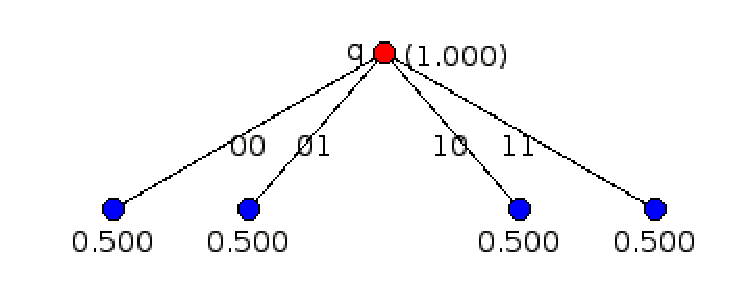
\includegraphics[scale=.6]{images/HadQbit.eps}
}
\caption{A \qbit{} after a \Had{} transform}\label{fig:lqplHadQbit}
\end{figure}

With multiple \qbit{}s,  the representation becomes hierarchical.
For example, two \qbit{s} will be represented by a tree with one of the
\qbits{} at the top and each of its sub-branches
 having the second \qbit{} below it. 
Consider applying a Hadamard transform to one \qbit, followed by a 
controlled-Not with that \qbit{} as the control. This is 
a standard way to entangle two \qbits. As illustrated in
\vref{fig:entangled}, this creates a tree in the quantum stack with
a total of four non-zero leaves. The quantum stack in the figure
corresponds to a sparse representation of the density matrix:

{\begin{singlespace}
\[\left[
\begin{array}{c|c}
\begin{array}{cc}
.5&0\\0&0
\end{array} &
\begin{array}{cc}
0&.5\\0&0
\end{array}\\
\hline
\begin{array}{cc}
0&0\\.5&0\\
\end{array} &
\begin{array}{cc}
0&0\\0&.5
\end{array}
\end{array}\right]
\]
\end{singlespace}
}

\begin{figure}[htbp]
\centerline{
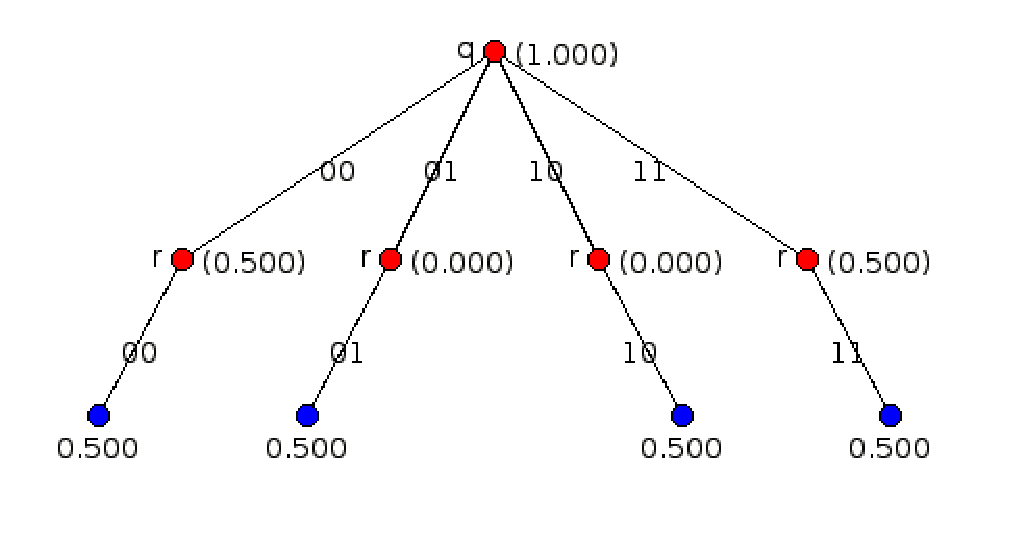
\includegraphics[scale=0.6]{images/entangledQbits.eps}
}
\caption{Two entangled \qbits}\label{fig:entangled}
\end{figure}

\subsection{Representation of integers and Boolean values}\label{subsec:representclassicaldata}
Numeric and Boolean
 data in the quantum stack machine is represented by a node with
a sub-branch for each value that occurs with a non-zero probability. 
These values may be of either integer or Boolean type.

\begin{figure}[htbp]
\centerline{
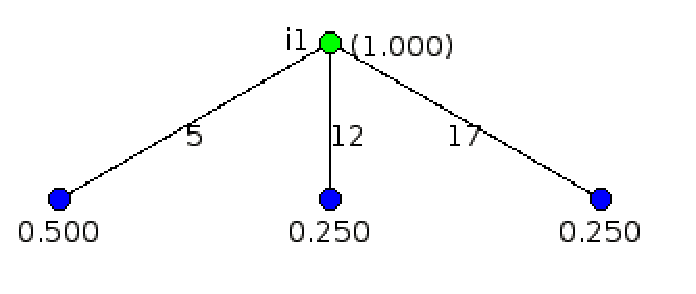
\includegraphics[scale=.6]{images/integer.eps}
}
\caption{An integer with three distinct values}\label{fig:integerofthree}
\end{figure}

\Vref{fig:integerofthree} depicts an
integer $i1$ which has 
a $50\%$ probability of being $5$, and $25\%$ each of being $12$ or $17$.

\subsection{Representation of general data types}\label{subsec:representgeneraldatatyps}
The general datatype is represented 
as a node with one branch for each of the constructors that occurs
with a non-zero probability. Each branch is labelled by the 
constructor and the names of any nodes that are 
bound to it\footnote{For example, in \qtype{List}s of 
integers, the
\qcons{Cons} constructor requires a base integer and another \qtype{List}.}.
These
nodes will be referred to as  \emph{bound nodes}.


\begin{figure}[htbp]
\centerline{
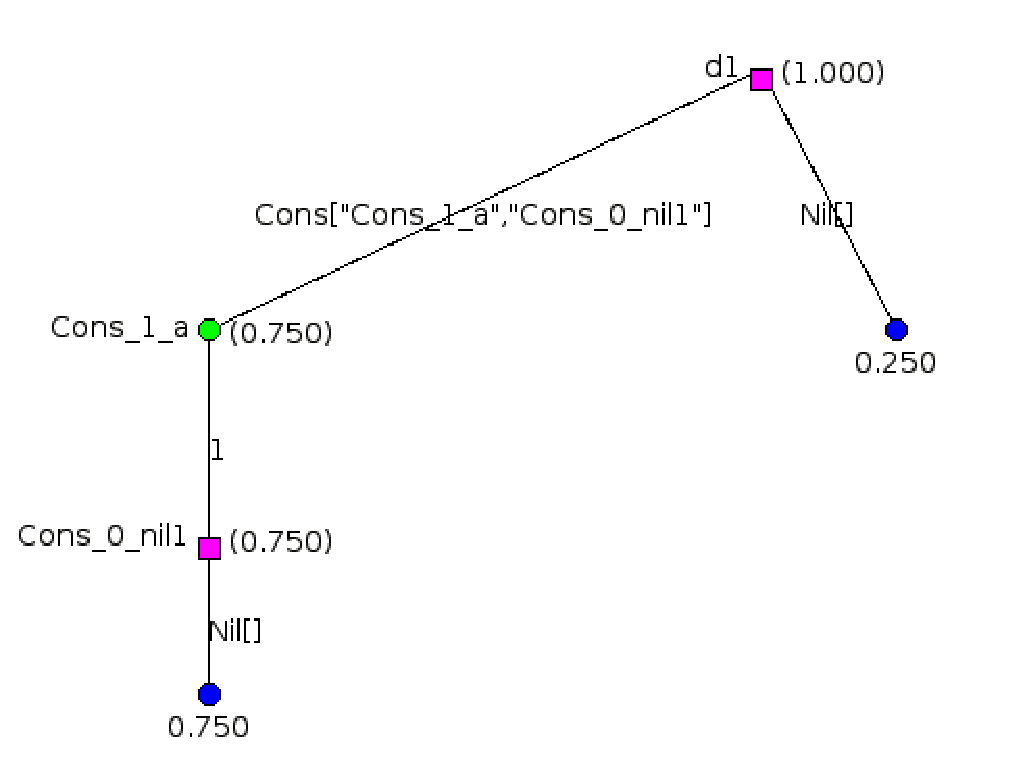
\includegraphics[scale=.5]{images/listExample.eps}
}
\caption{A list which is a mix of $[\ ]$ and $[1]$.}\label{fig:schizolist}
\end{figure}



For example, in the \qtype{List} that appears in \vref{fig:schizolist}, 
the top node  is a mix of values. The node $d1$ has a $25\%$ chance of 
being \qcons{Nil} and $75\%$ of being a \qcons{Cons} of two bound nodes.
The first bound node is an element of the base type, integer. 
It is labelled \terminalio{Cons\_1\_a} which
is an integer node having the single value 1. The second bound element is 
\terminalio{Cons\_0\_nil1},  which is another list having the
 single value of \qcons{Nil}. 




